\documentclass[landscape]{article}
\usepackage{multicol}
\usepackage[margin=1in]{geometry}
\usepackage{clrscode3e}
\usepackage{amsmath}
\usepackage{graphicx}

\newcommand{\bi}{\begin{itemize}}
\newcommand{\ii}{\item}
\newcommand{\ei}{\end{itemize}}
\newcommand{\bn}{\begin{enumerate}}
\newcommand{\en}{\end{enumerate}}
\newcommand{\set}[1]{\ensuremath{\left\{#1\right\}}}
\newcommand{\pr}[1]{\ensuremath{\mbox{Pr}\left\{#1\right\}}}
\newcommand{\flr}[1]{\ensuremath{\left\lfloor#1\right\rfloor}}
\newcommand{\ceil}[1]{\ensuremath{\left\lceil#1\right\rceil}}

\newcommand{\sect}[1]{\newpage{\textbf{#1}}}

\setlength{\parindent}{0in}

\newcommand{\nop}[1]{}

\title{Notes on Hash Tables}
\author{Geoffrey Matthews}
\begin{document}
\maketitle
\titlepage
\huge


\sect{Dictionary Operations}
\bi
\ii \textsc{Insert}
\ii \textsc{Search}
\ii \textsc{Delete}
\ei

\sect{Hash table implementation of Dictionary}
\bi
\ii Expected search time: $O(1)$
\ii Worst case search: $O(n)$
\ei

\sect{Hash table is generalization of an ordinary array}
\bi
\ii With array, the key $k$ is the position $k$ in the array.
\ii Given a key $k$, we find the element with key $k$
by \textbf{direct addressing}.
\ii Direct addressing only applicable when we can afford to
allocate an array with one position for every key.
\ei

\sect{Use hash table when we don't have one position for each key}
\bi
\ii Number of keys stored is small relative to the number of possible
keys.
\ii Hash table is an array with size proportional to the number of
keys stored, not the number of possible keys.
\ii Given a key $k$, don't use $k$ to index the array.
\ii Instead, compute a function of $k$ and use that to index the
array.
\ii This function is called a \textbf{hash function}.
\ii Have to solve issue of what to do when hash function maps multiple
keys to same table entry.
\bi\ii chaining \ii open addressing \ei
\ii We will not discuss open addressing.
\ei

\sect{Direct-address tables}
\bi
\ii Scenario:
\bi
\ii Maintain a dynamic set
\ii Each element has a key drawn from a universe
$U=\{0,1,\ldots,m-1\}$ where $m$ isn't too large.
\ii No two elements have the same key.
\ei
\ii Represent by a \textbf{direct-address table}, or array, $T[0\ldots
  m-1]$:
\bi
\ii Each \textsl{slot}, or position, corresponds to a key in $U$.
\ii If there's an element $x$ with key $k$, then $T[k]$ contains a
pointer to $x$.
\ii Otherwise, $T[k]$ is empty, represented by \textsc{NIL}.
\ei
\ei



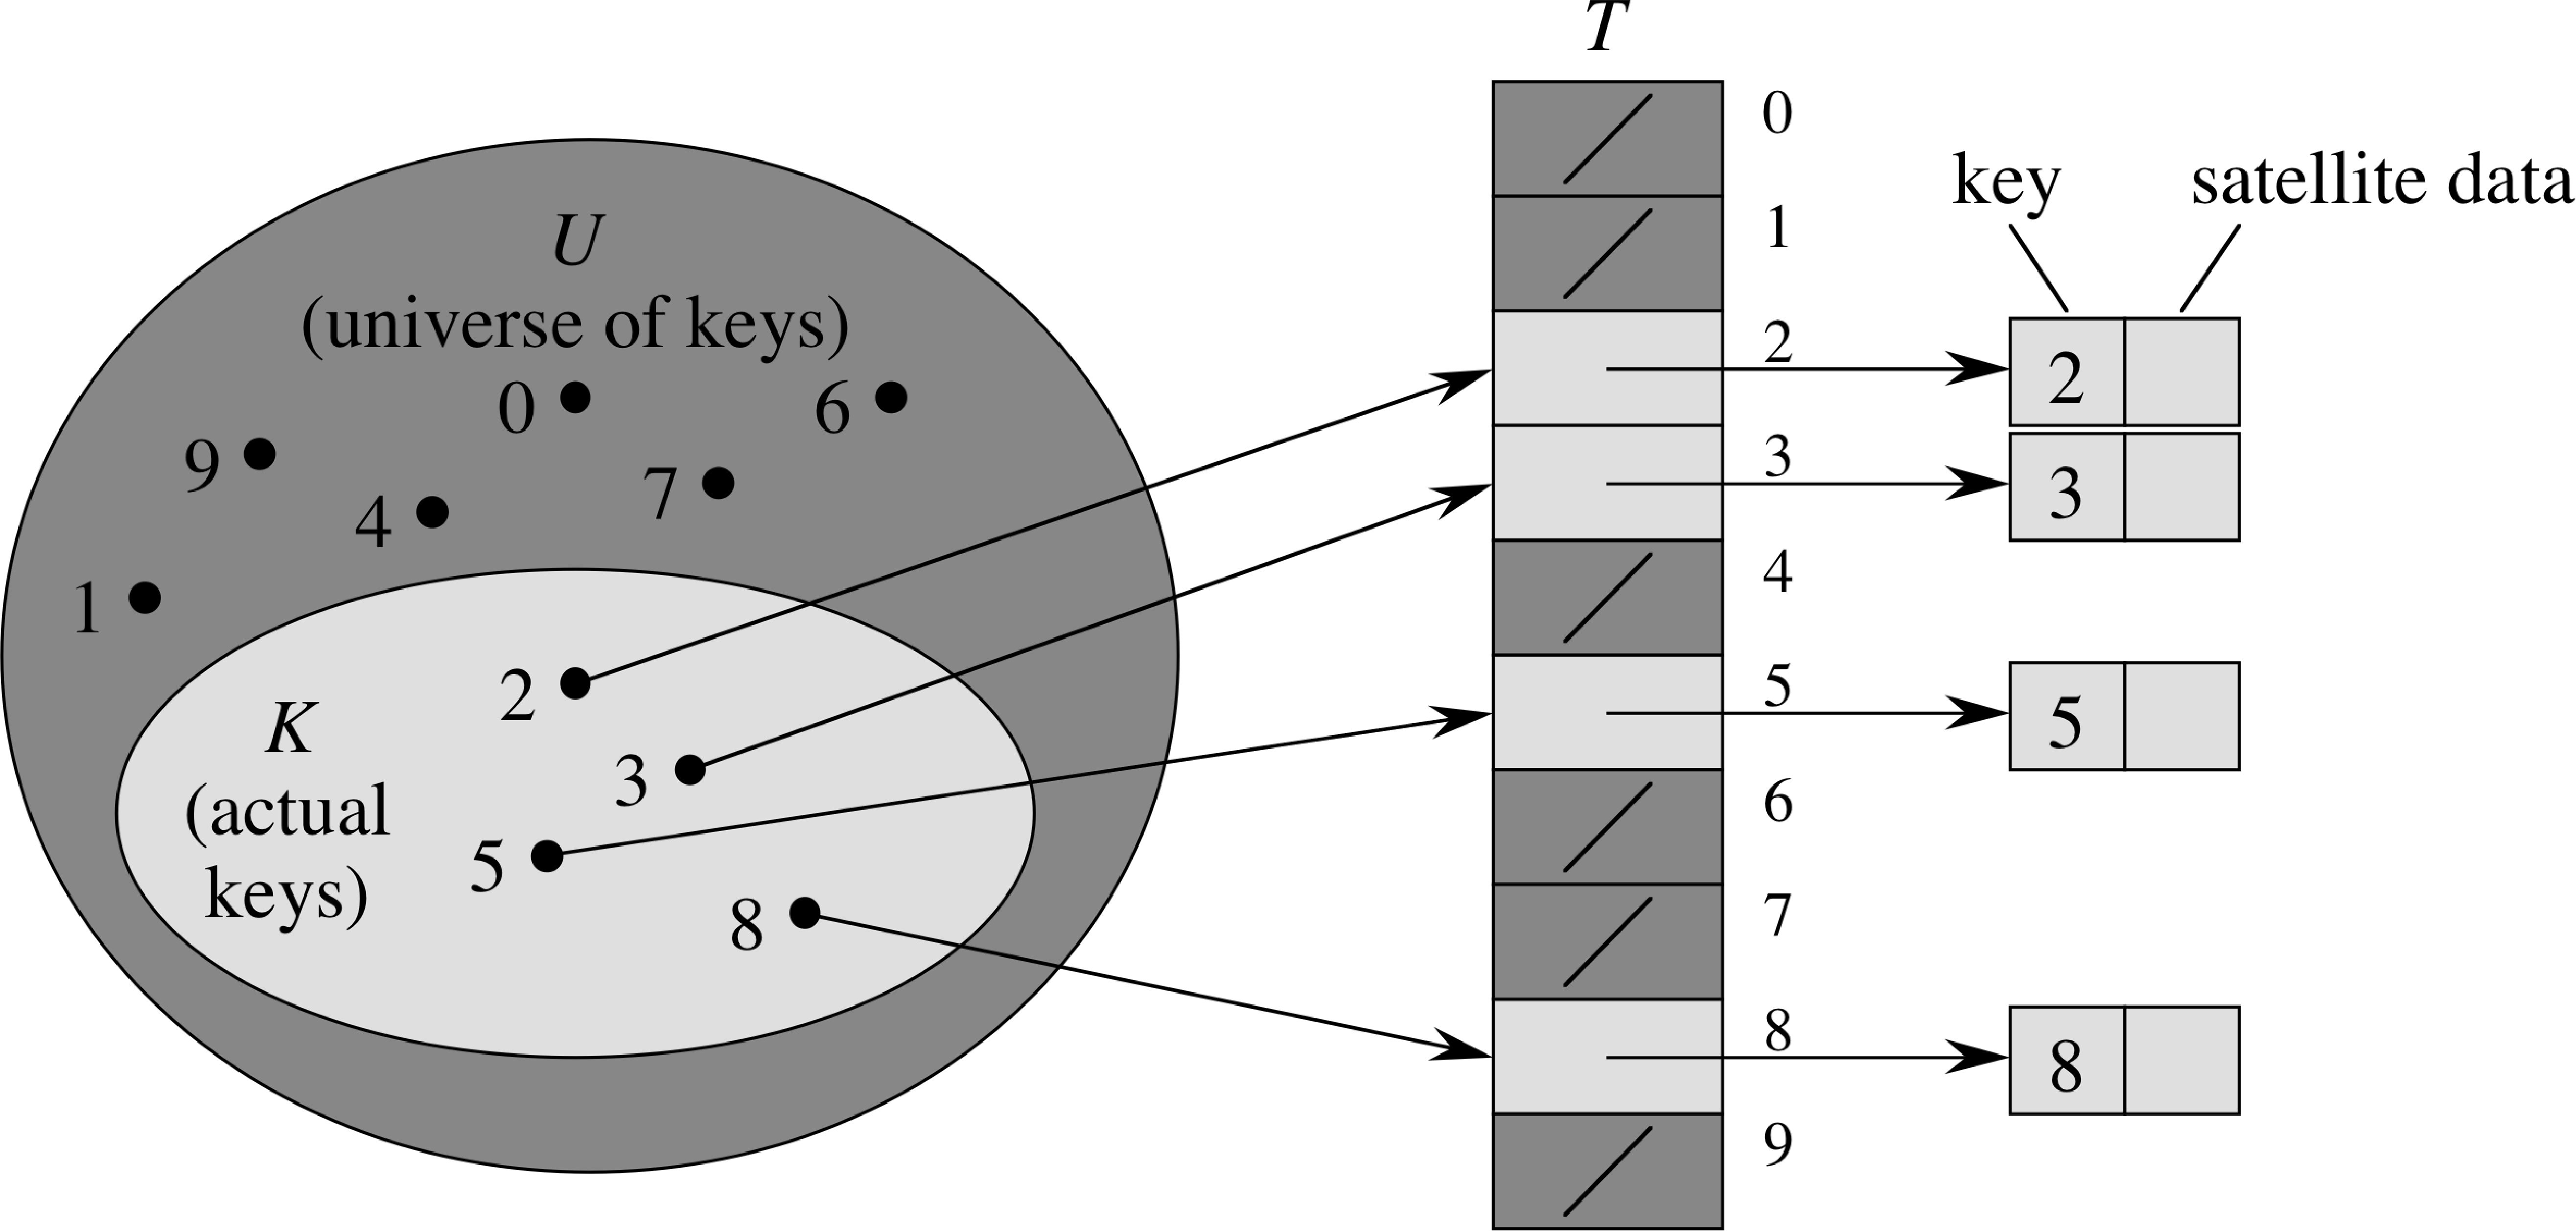
\includegraphics[width=\textwidth]{Fig-11-1.pdf}
\begin{multicols}{2}
\begin{codebox}
  \Procname{Direct-Address-Search(T,k)}
  \li \Return $T[k]$
\end{codebox}
\begin{codebox}
  \Procname{Direct-Address-Insert(T,k)}
  \li $T[key[x]] = x$
\end{codebox}
\begin{codebox}
  \Procname{Direct-Address-Delete(T,k)}
  \li $T[key[x]] = \textsc{nil}$
\end{codebox}
All operations $O(1)$.
\end{multicols}

\sect{Hash tables}
\bi
\ii If $U$ is large, storing a table of size $|U|$ is impractical.
\ii Often the set $K$ of keys actually used is small compared to $U$.
\bi\ii Most of the space in a direct-access table is wasted.\ei
\ii When $K$ is much smaller than $U$, a hash table requires much less
space than a direct-address table.
\ii Can reduce storage requirements to $\Theta(|K|)$
\ii Can still get $O(1)$ search time on {\em average}, but not {\em
  worst} case.
\ei

\sect{Hash table idea}
\bi
\ii Instead of storing an element with key $k$ in slot $k$,
use a function $h$ and store the element in slot $h(k)$.
\ii $h$ is called a \textbf{hash function}
\ii $h: U \rightarrow \{0,1,\ldots,m-1\}$
\ii $m \ll |U|$
\ii $h(k)$ is a legal slot number in $T$
\ii We say $k$ {\em hashes} to $h(k)$
\ei

\sect{Collisions}

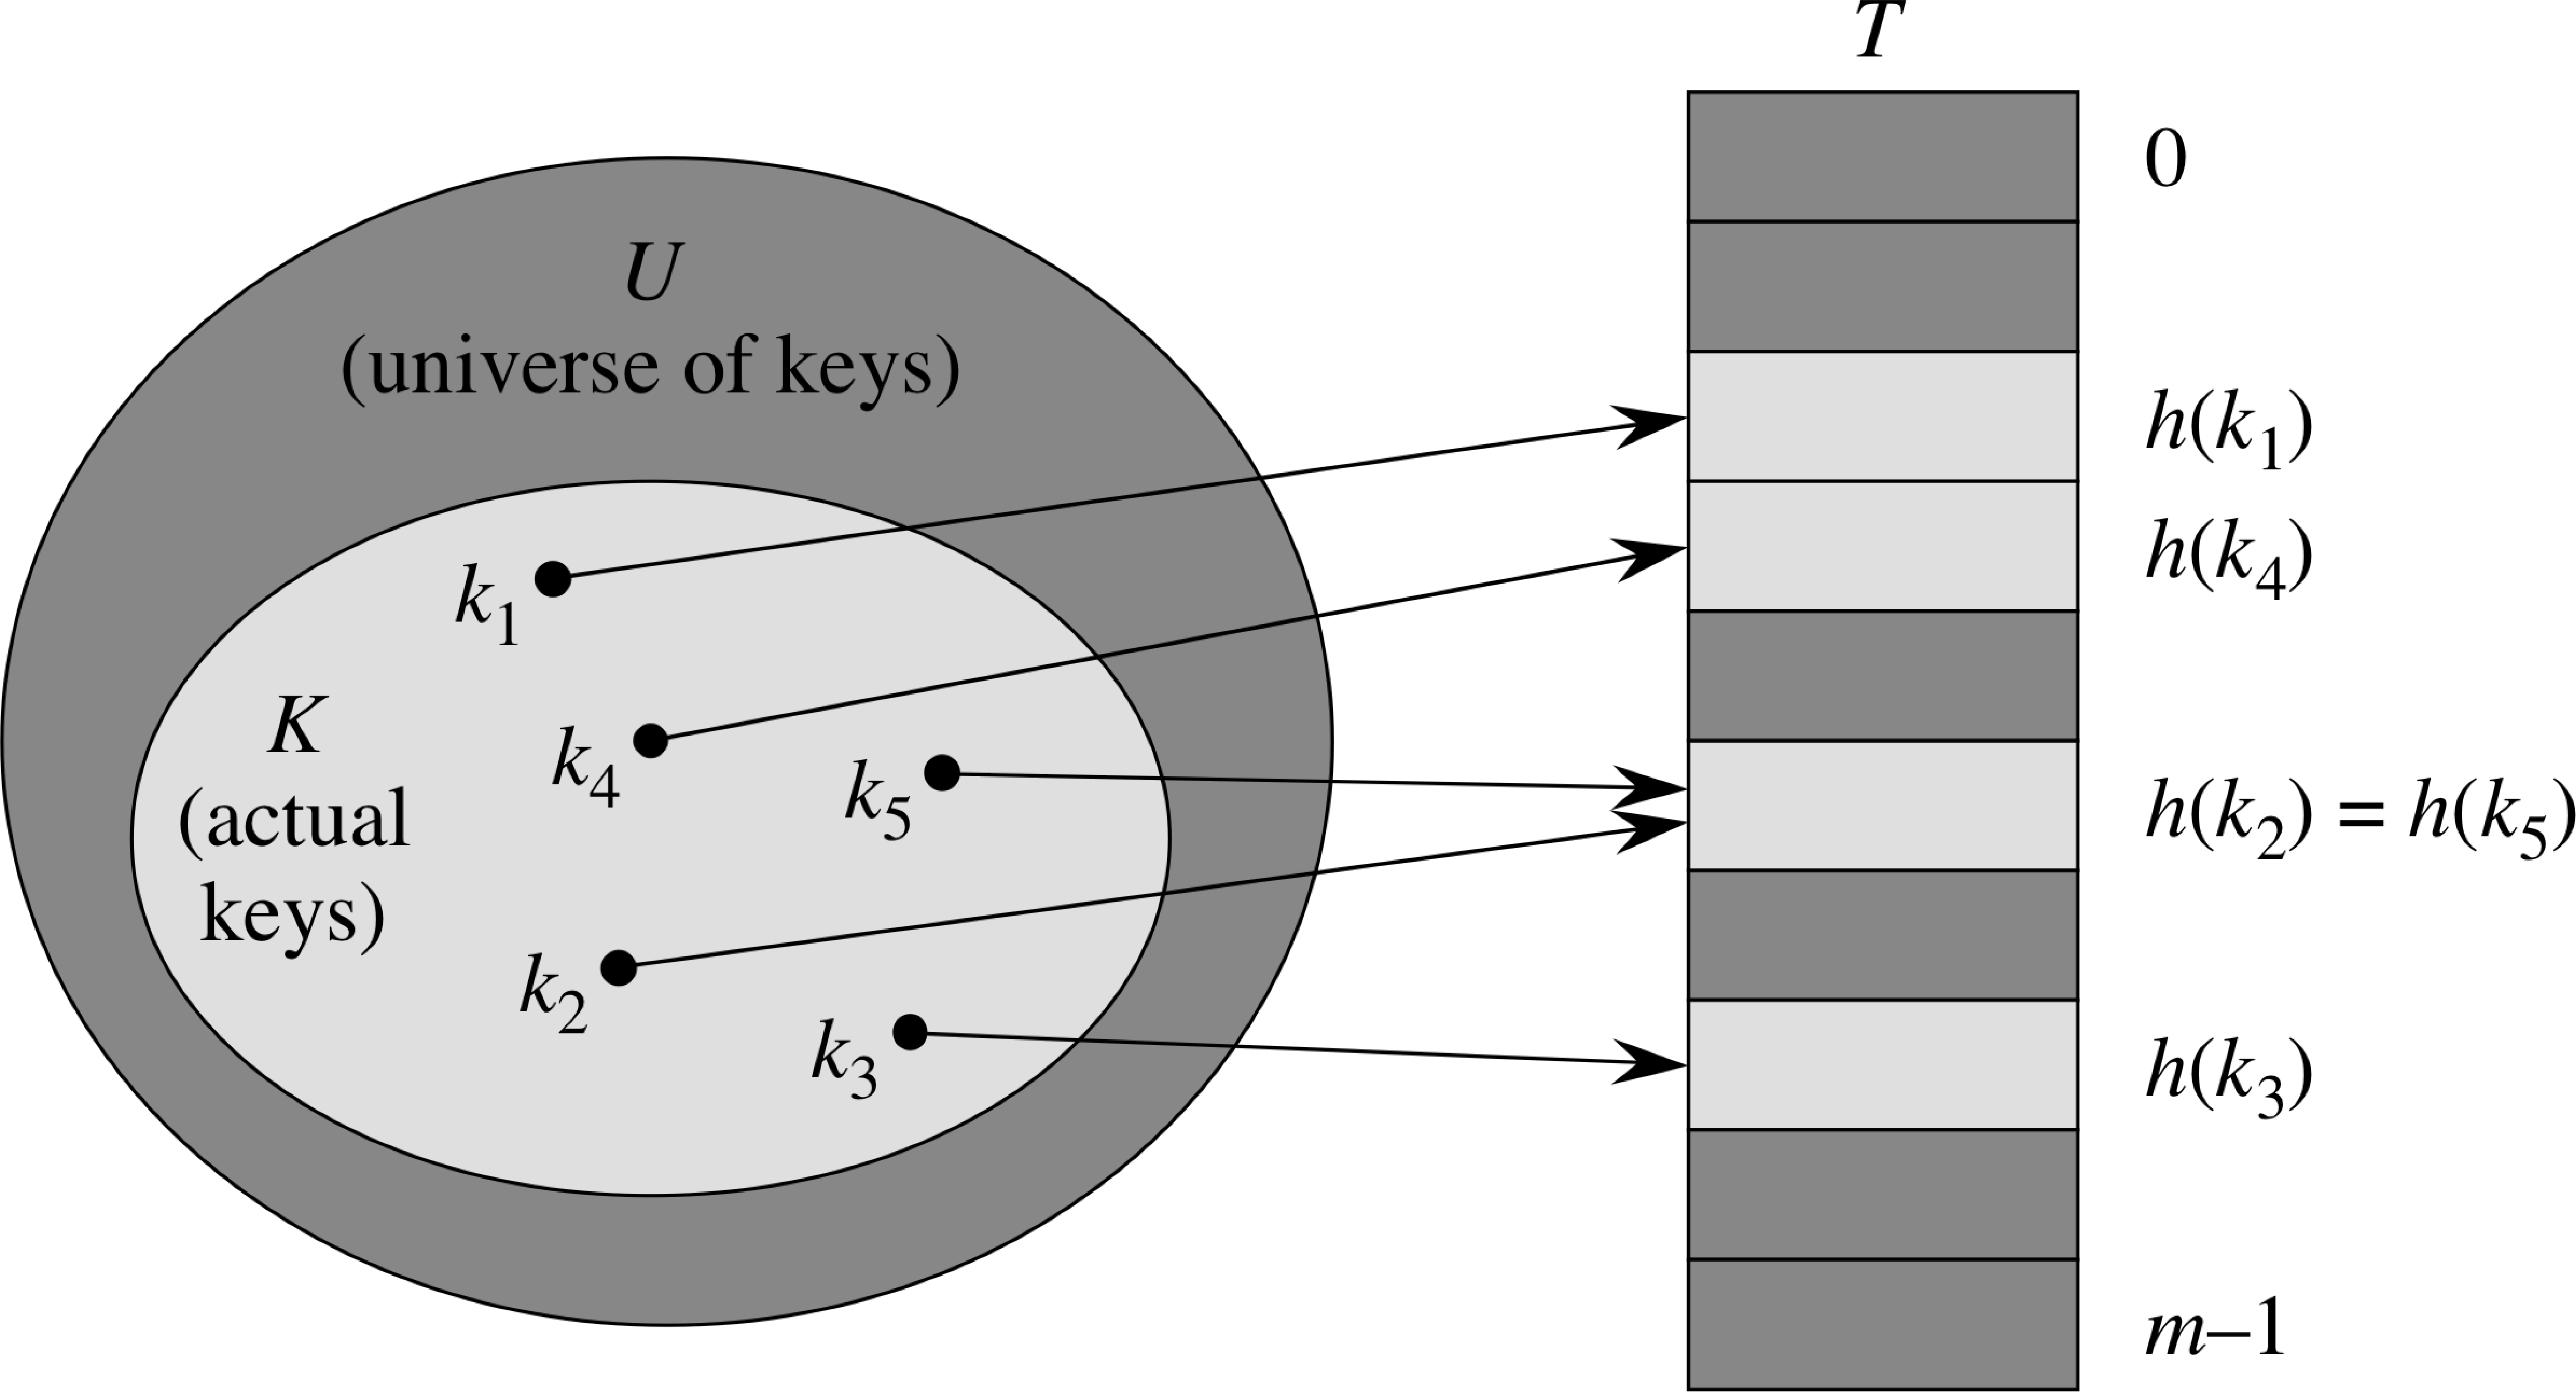
\includegraphics[width=\textwidth]{Fig-11-2.pdf}

\sect{Collisions}
\bi
\ii When two or more keys hash to the same slot.
\ii Can happen when there are more possible keys than slots ($|U| >
m$).
\ii For a given set $K$ of keys with $|K|\leq m$, may or may not
happen.
\ii Definitely happens when $|K| > m$.
\ii Must be prepared to handle collisions in all cases.
\ii Two methods:
\bi \ii chaining \ii open addressing \ei
\ii Chaining is usually better.
\ii We will not discuss open addressing.
\ei


\sect{Collision resolution by chaining}
\bi
\ii Put all elements that hash to the same slot into a linked list.
\ei

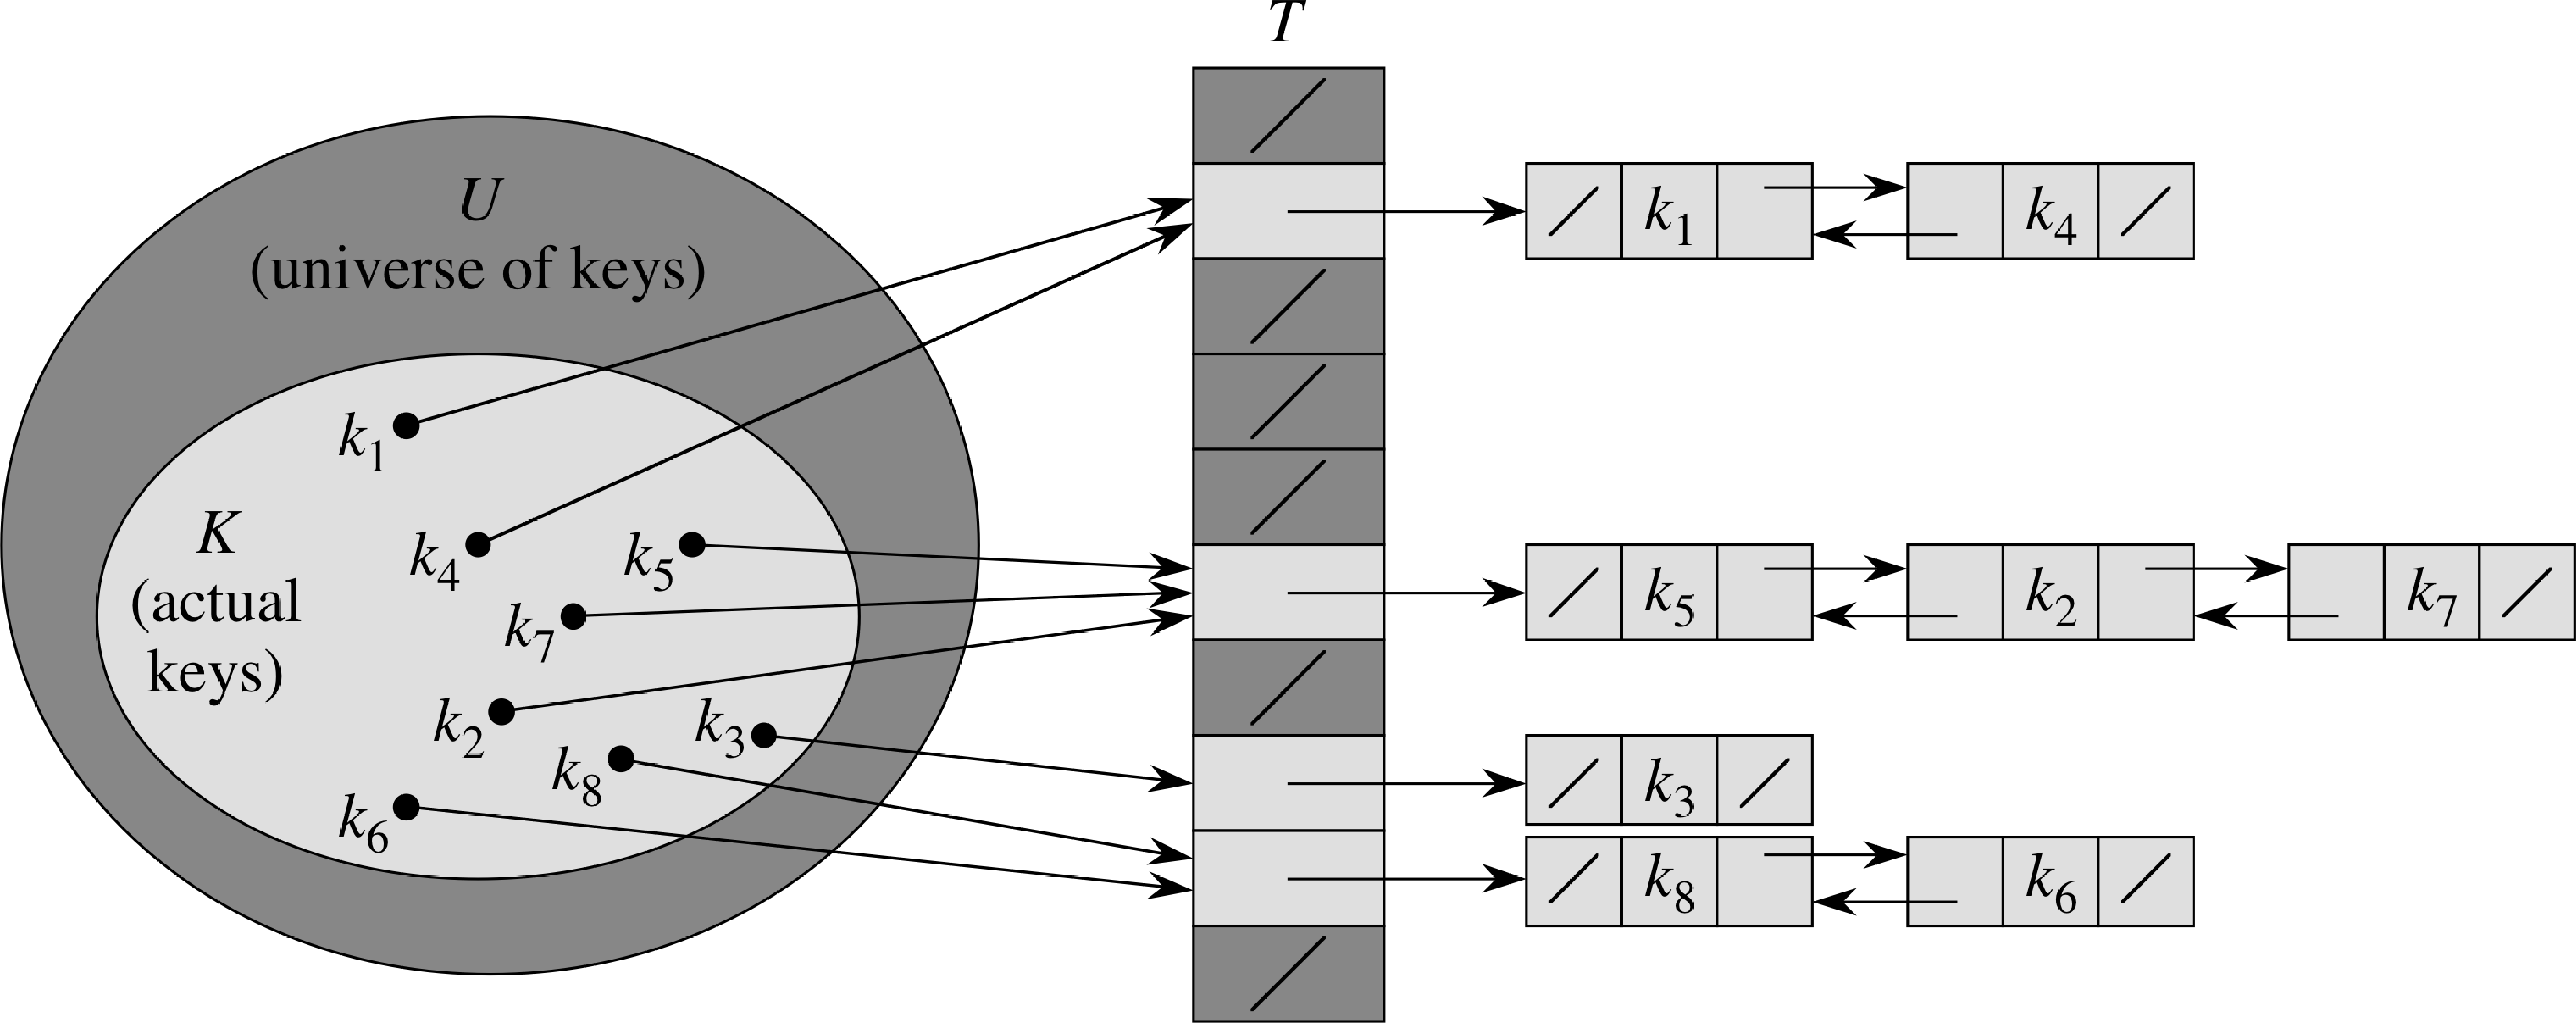
\includegraphics[width=\textwidth]{Fig-11-3.pdf}

\bi
\ii Doubly linked list allows easy deletion.
\ei

\sect{Implementation of heap with chaining}
\begin{description}
  \ii[Insertion:]\mbox{}

  \begin{codebox}
    \Procname{Chained-Hash-Insert$(T,x)$}
    \li insert $x$ at the head of list $T[h(key[x])]$
  \end{codebox}
  \bi
  \ii Worst case $O(1)$
  \ii Assumes element inserted not already in list.
  \ii Would take an additional search to see if it was already
  inserted.
  \ei

\end{description}

\sect{Implementation of heap with chaining}
\begin{description}
  \ii[Search:]\mbox{}

  \begin{codebox}
    \Procname{Chained-Hash-Search$(T,k)$}
    \li search for element with key $k$ in list $T[h(k)]$
  \end{codebox}
  \bi
  \ii Running time proportional to length of list in slot $h(k)$
  \ei

\end{description}

\sect{Implementation of heap with chaining}
\begin{description}
  \ii[Deletion:]\mbox{}

  \begin{codebox}
    \Procname{Chained-Hash-Delete$(T,x)$}
    \li delete $x$ from the list $T[h(key[x])]$
  \end{codebox}
  \bi
  \ii Given pointer $x$ to the element to delete, so no search
  is needed to find this element.
  \ii Worst case $O(1)$ if lists are doubly linked.
  \ii If lists are singly linked, deletion takes as long as search,
  because we must find $x$'s predecessor.
  \ei

\end{description}

\sect{Analysis of hashing with chaining}
\bi
\ii Given a key, how long does it take to find an element with that
key, or determine that there is no element with that key?
\ii Analysis is in terms of the \textbf{load factor} $\alpha = n/m$
\ii $n = $\# elements in the table
\ii $m = $\# slots in the table
\ii Load factor is average number of elements per linked list.
\ii Can have $\alpha < 1$, $\alpha = 1$, or $\alpha > 1$
\ii Worst case is when all $n$ keys hash to the same slot:
\bi
\ii a single list of length $n$
\ii worst case is $\Theta(n)$ plus time to compute $h$
\ei
\ii Average case depends on how well the hash function distributes
keys among slots.
\ei

\sect{Average-case analysis of hashing with chaining}
\bi
\ii Assume \textbf{simple uniform hashing}: any given element is
equally likely to hash to any of the $m$ slots.
\ii For $j=0,1,\ldots,m-1$, denote the length of the list $T[j]$ by
$n_n$.
\ii $n=n_0+n_1+\cdots+n_{m-1}$
\ii Average value of $n_j$ is $E[n_j] = \alpha = n/m$
\ii Assume we can compute $h$ in $O(1)$ time, so that the time
required to search for $k$ depends on the length $n_{h(k)}$ of the
list $T[h(k)]$.
\ii Two cases:
\bi
\ii Unsuccessful search:  hash table has no element with key $k$
\ii Successful search:  hash table contains an element with key $k$
\ei
\ei

\sect{Unsuccessful search}

\begin{description}
\item[Theorem] \mbox{}

  An unsuccessful search takes expected time
    $\Theta(1+\alpha)$.

  \item[Proof]\mbox{}
    \bi
    \ii Simple uniform hashing means any key not already in the table
    is equally likely to hash to any of the $m$ slots.
    \ii To search unsuccessfully for any key $k$, need to search to
    the end of the list $T[h(k)]$.
    \ii This list has expected length $\alpha$.
    \ii Adding the time to compute the hash function gives
    $\Theta(1+\alpha)$.
    \ei
\end{description}

\sect{Successful search}

\bi
\ii The expected time for a successful search is also
$\Theta(1+\alpha)$.
\ii The probability that each list is searched is proportional to the
length of the list.
\ei

\sect{Successful search}
\begin{description}
\item[Theorem] \mbox{}

  A successful search takes expected time
    $\Theta(1+\alpha)$.

  \item[Proof]\mbox{}
    \bi
    \ii Assume the element $x$ is equally likely to be any of the $n$
    elements stored in the table.
    \ii The number of elements examined during the search for $x$ is 1
    more than the number of elements that appear before $x$ in $x$'s
    list.
    \ii These are the elements inserted {\em after} $x$ was inserted.
    \ii We need to find the average, over $n$ elements $x$ in the
    table, how many elements were inserted into $x$'s list after $x$
    was inserted.
    \ii For $i=1,2,...,n$, let $x_i$ be the $i$th element inserted,
    and let $k_k = key[x_i]$.
    \ii For all $i$ and $j$ define
    \[ X_{ij} = \textbf{I}\{h(k_i) = h(k_j)\}\]
    \ii Simple uniform hashing means
    \[ Pr\{h[k_k)=h(k_j)\} = 1/m = E[X_{ij}]\]
    \ei
\end{description}

\sect{Expected number of elements examined in successful search}
\begin{align*}
  E\left[\frac{1}{n}\sum_{i=1}^{n}\left(1+\sum_{j=i+1}^{n}X_{ij}\right)\right]
  &=
  \frac{1}{n}\sum_{i=1}^{n}\left(1+\sum_{j=i+1}^{n}E[X_{ij}]\right)\\
  &=
  \frac{1}{n}\sum_{i=1}^{n}\left(1+\sum_{j=i+1}^{n}\frac{1}{m}\right)\\
  &=
  1+\frac{1}{nm}\sum_{i=1}^{n}(n-i)\\
  &=
  1+\frac{1}{nm}\sum_{i=0}^{n-1}i\\
  &=
  1+\frac{1}{nm}\frac{n(n-1)}{2}\\
  &=
  1+\frac{n-1}{2m}\\
  &= 1 + \frac{\alpha}{2} - \frac{\alpha}{2n} \\ &= \Theta(1+\alpha)
\end{align*}

\sect{Alternative analysis}
\bi
\ii $X_{ij\ell} = \textbf{I}\{\mbox{the search is for $x_i$,
  $h(k_i)=h(k_j)=\ell$\}}$
\ii Simple uniform hashing means $Pr\{h(k_i)=\ell\}=Pr\{h(k_j)=\ell\}=
1/m$
\ii $Pr\{\mbox{the search is for $x_i$}\} = 1/n$
\ii All these are independent: $Pr\{X_{ij\ell}=1\} =
\textbf{E}[X_{ij\ell}] =1/nm^2 $
\begin{align*}
Y_j &= \textbf{I}\{\mbox{$x_j$ appears in a list prior to the
  $x_i$}\}\\
   &= \sum_{i=1}^{j-1}\sum_{\ell=0}^{m-1} X_{ij\ell}
\end{align*}
\ei

\sect{Alternative analysis, continued}
\begin{align*}
  E\left[1+\sum_{j=1}^n Y_j\right]
  &=
  1 + E\left[\sum_{j=1}^{n}\sum_{i=1}^{j-1}\sum_{\ell=0}^{m-1} X_{ij\ell}\right]\\
  &=
  1 + \sum_{j=1}^{n}\sum_{i=1}^{j-1}\sum_{\ell=0}^{m-1} E[X_{ij\ell}]\\
  &=
  1 + \sum_{j=1}^{n}\sum_{i=1}^{j-1}\sum_{\ell=0}^{m-1} \frac{1}{nm^2}\\
  &=
  1 + {n \choose 2}\cdot m \cdot \frac{1}{nm^2}\\
  &=
  1 + \frac{n-1}{2m}\\
  &=
  1 + \frac{\alpha}{2} - \frac{\alpha}{2n} = \Theta(1 + \alpha)
\end{align*}


\sect{Interpretation}
\bi
\ii If $n=O(m)$ then $\alpha = n/m = O(1)$, which means searching
takes constant time on average.
\ii Since insertion  and deletion take $O(1)$ worst case time,
all dictionary operations take average time $O(1)$.
\ei

\sect{Hash functions}
\bi
\ii Ideally, satisfies the assumption of simple uniform hashing.
\ii In practice, impossible since we don't know the
distribution of input keys.
\ii In practice, many functions work OK.
\ei

\sect{Keys as natural numbers}
\bi
\ii Can interpret any computer data as natural number.
\ii Strings, for example: \textsc{CLRS}
\bi
\ii ASCII: 67, 76, 82, 83
\ii There are 128 ASCII values
\ii $h(\textsc{CLRS}) = 67(128^3) + 76(128^2) + 82(128^1) + 83(128^0) = 141,764,947$
\ei
\ei

\sect{Division method for hash functions}
\[ h(k) = k \mbox{ mod } m \]
\bi
\ii Fast
\ii Powers of 2 are bad values for $m$, just uses least significant bits.
\ii Good choice for $m$:  prime number not too close to a power of 2.
\ei

\sect{Multiplication method for hash functions}
  \[h(k) = \lfloor m ((kA) \mbox{ mod } 1)\rfloor\]

\begin{enumerate}
\item Choose $A$ in range $0<A<1$.
\item Take fractional part of $kA$.
\item Multiply by $m$.
\item Take floor.
\end{enumerate}
\bi
\ii Slower than division method.
\ii Value of $m$ is not critical.
\bi\ii Can even use $m=2^p$\ei 
\ii Knuth suggests a good value for $A\approx (\sqrt{5} -1)/2$
\ei


\sect{Open addressing}
\bi
\ii Store all keys in hash table, no linked lists.
\ii Use $i+1$ until we find an empty cell.
\ei
Example:  $h(n) = n\mod 10$  (really bad hash function)\\

\begin{minipage}{0.60\textwidth}
\begin{enumerate}
  \item Insert 12:
\begin{tabular}{|c|c|c|c|c|c|c|c|c|c|}\hline
  0&1&2&3&4&5&6&7&8&9\\\hline
{\sf x} &{\sf x} &12 &{\sf x} &{\sf x} &{\sf x} &{\sf x} &{\sf x} &{\sf x} &{\sf x} \\\hline
  \end{tabular}

  \item Insert 14:
\begin{tabular}{|c|c|c|c|c|c|c|c|c|c|}\hline
  0&1&2&3&4&5&6&7&8&9\\\hline
{\sf x} &{\sf x} &12 &{\sf x} &14 &{\sf x} &{\sf x} &{\sf x} &{\sf x} &{\sf x} \\\hline
  \end{tabular}

  \item Insert 32:
\begin{tabular}{|c|c|c|c|c|c|c|c|c|c|}\hline
  0&1&2&3&4&5&6&7&8&9\\\hline
{\sf x} &{\sf x} &12 &32 &14 &{\sf x} &{\sf x} &{\sf x} &{\sf x} &{\sf x} \\\hline
  \end{tabular}

  \item Insert 92:
\begin{tabular}{|c|c|c|c|c|c|c|c|c|c|}\hline
  0&1&2&3&4&5&6&7&8&9\\\hline
{\sf x} &{\sf x} &12 &32 &14 &92 &{\sf x} &{\sf x} &{\sf x} &{\sf x} \\\hline
  \end{tabular}

  \item Insert 53:
\begin{tabular}{|c|c|c|c|c|c|c|c|c|c|}\hline
  0&1&2&3&4&5&6&7&8&9\\\hline
{\sf x} &{\sf x} &12 &32 &14 &92 &53 &{\sf x} &{\sf x} &{\sf x} \\\hline
  \end{tabular}

\end{enumerate}
\end{minipage}
\begin{minipage}{0.40\textwidth}

\bi
\ii Linear probing leads to
\bi\ii\textbf{primary clustering}.\ei
\ii Better:
\bi \ii quadratic probing \ii double hashing \ei
\ii
Expected number of probes \[\frac{1}{1-\alpha}\]
\ei
\end{minipage}


%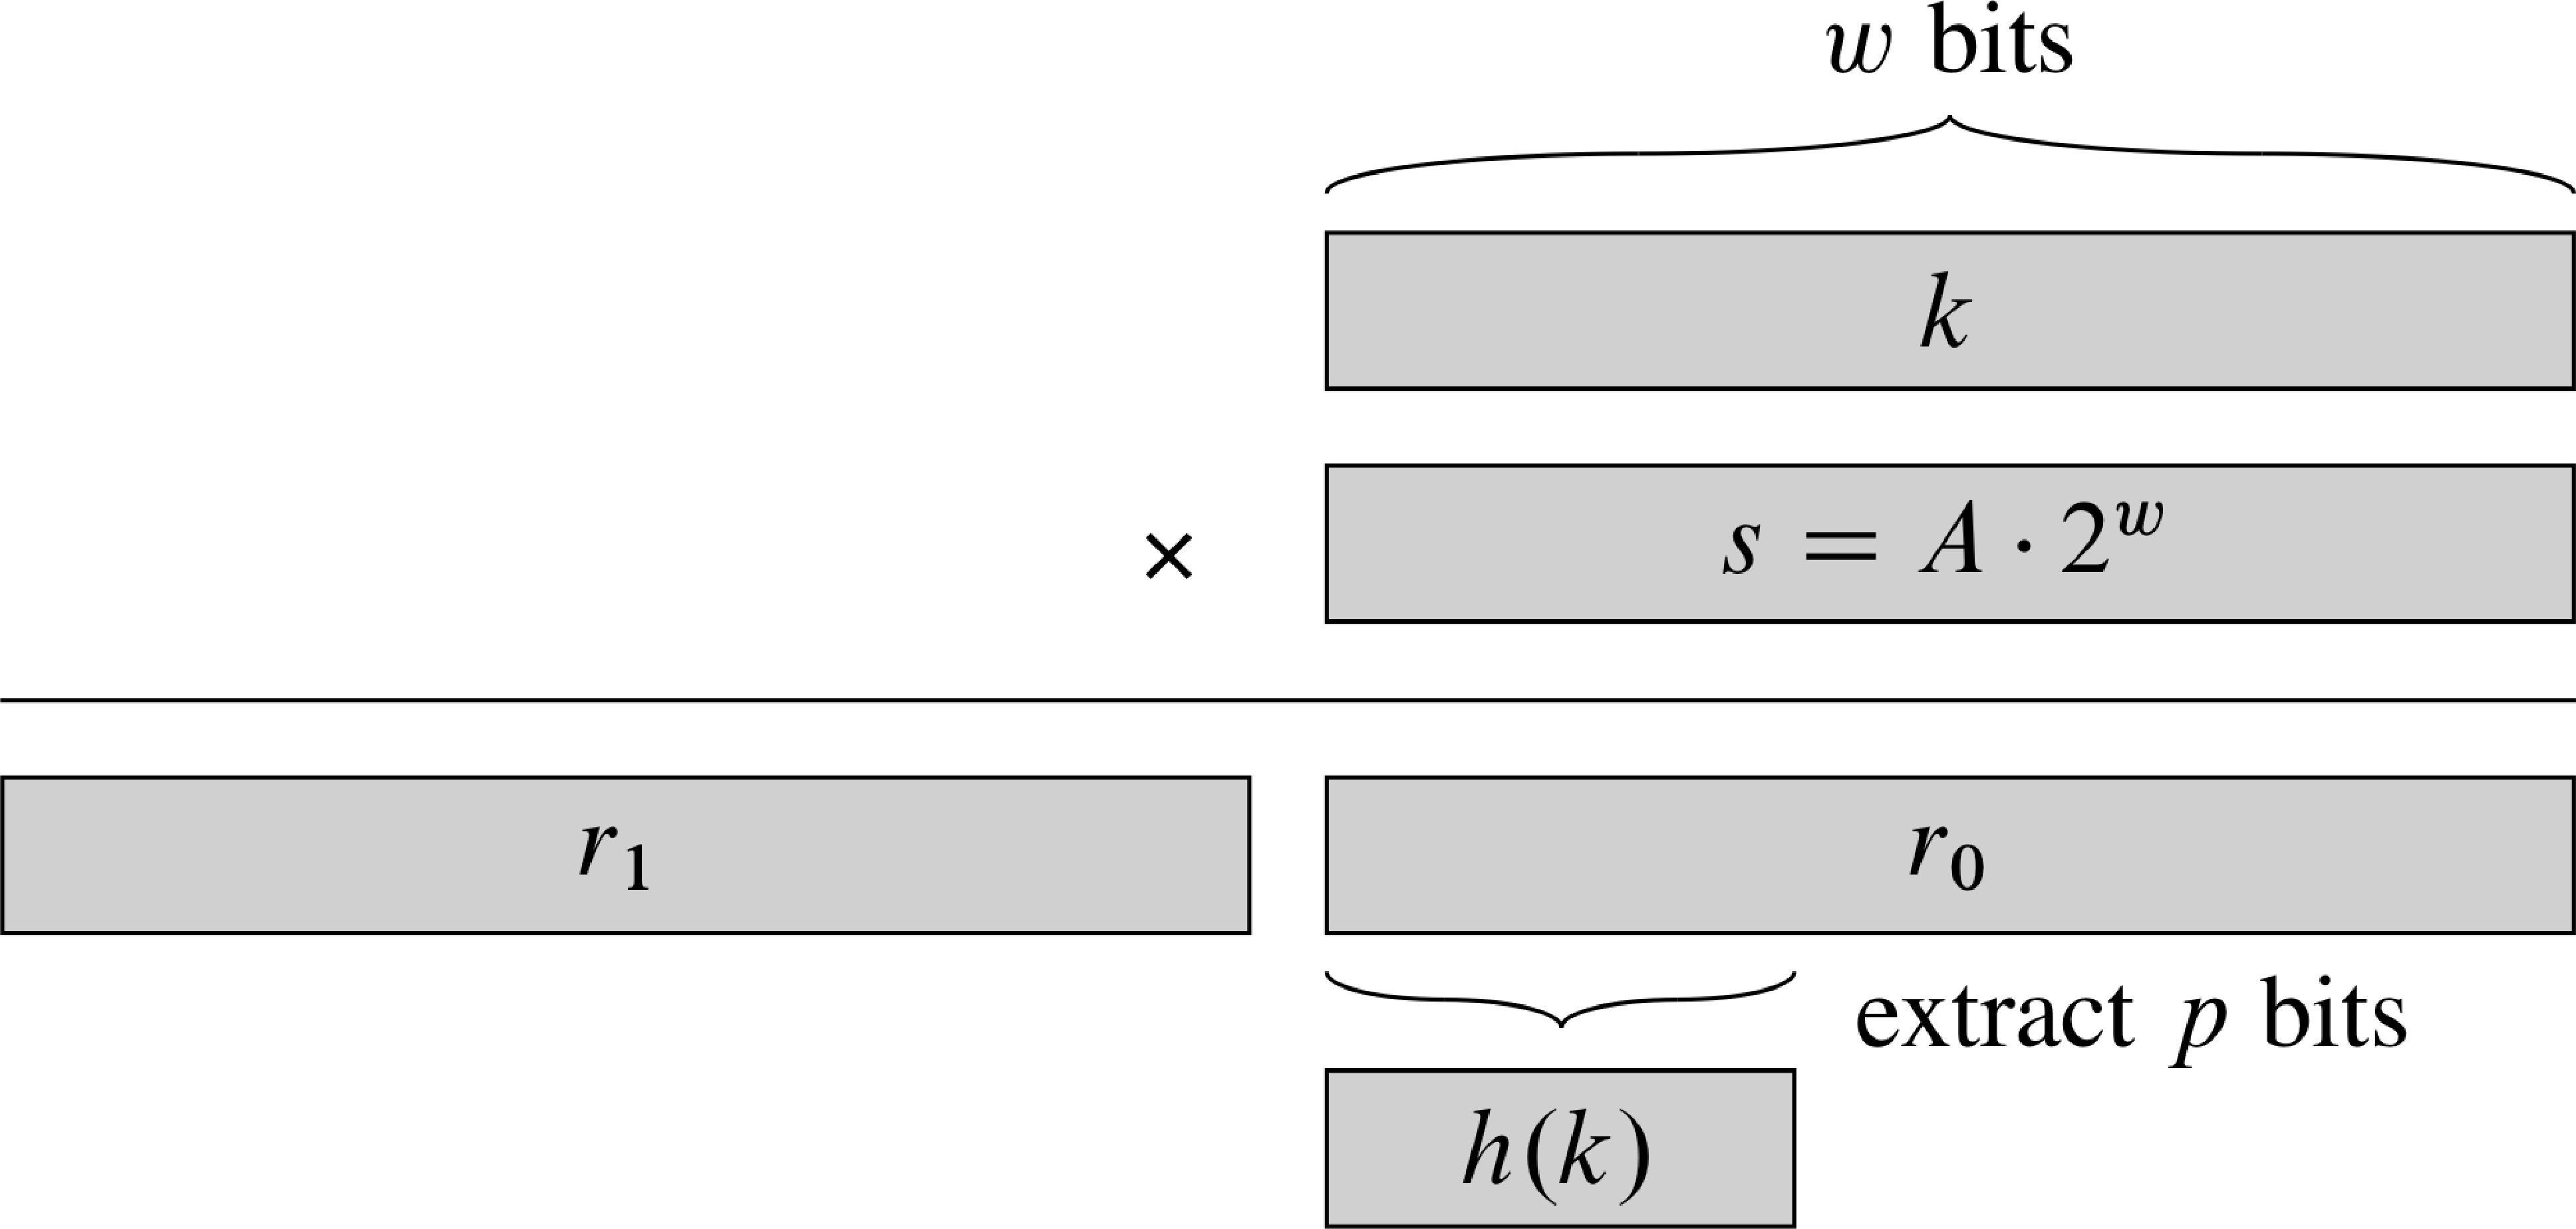
\includegraphics[width=\textwidth]{Fig-11-4.pdf}
%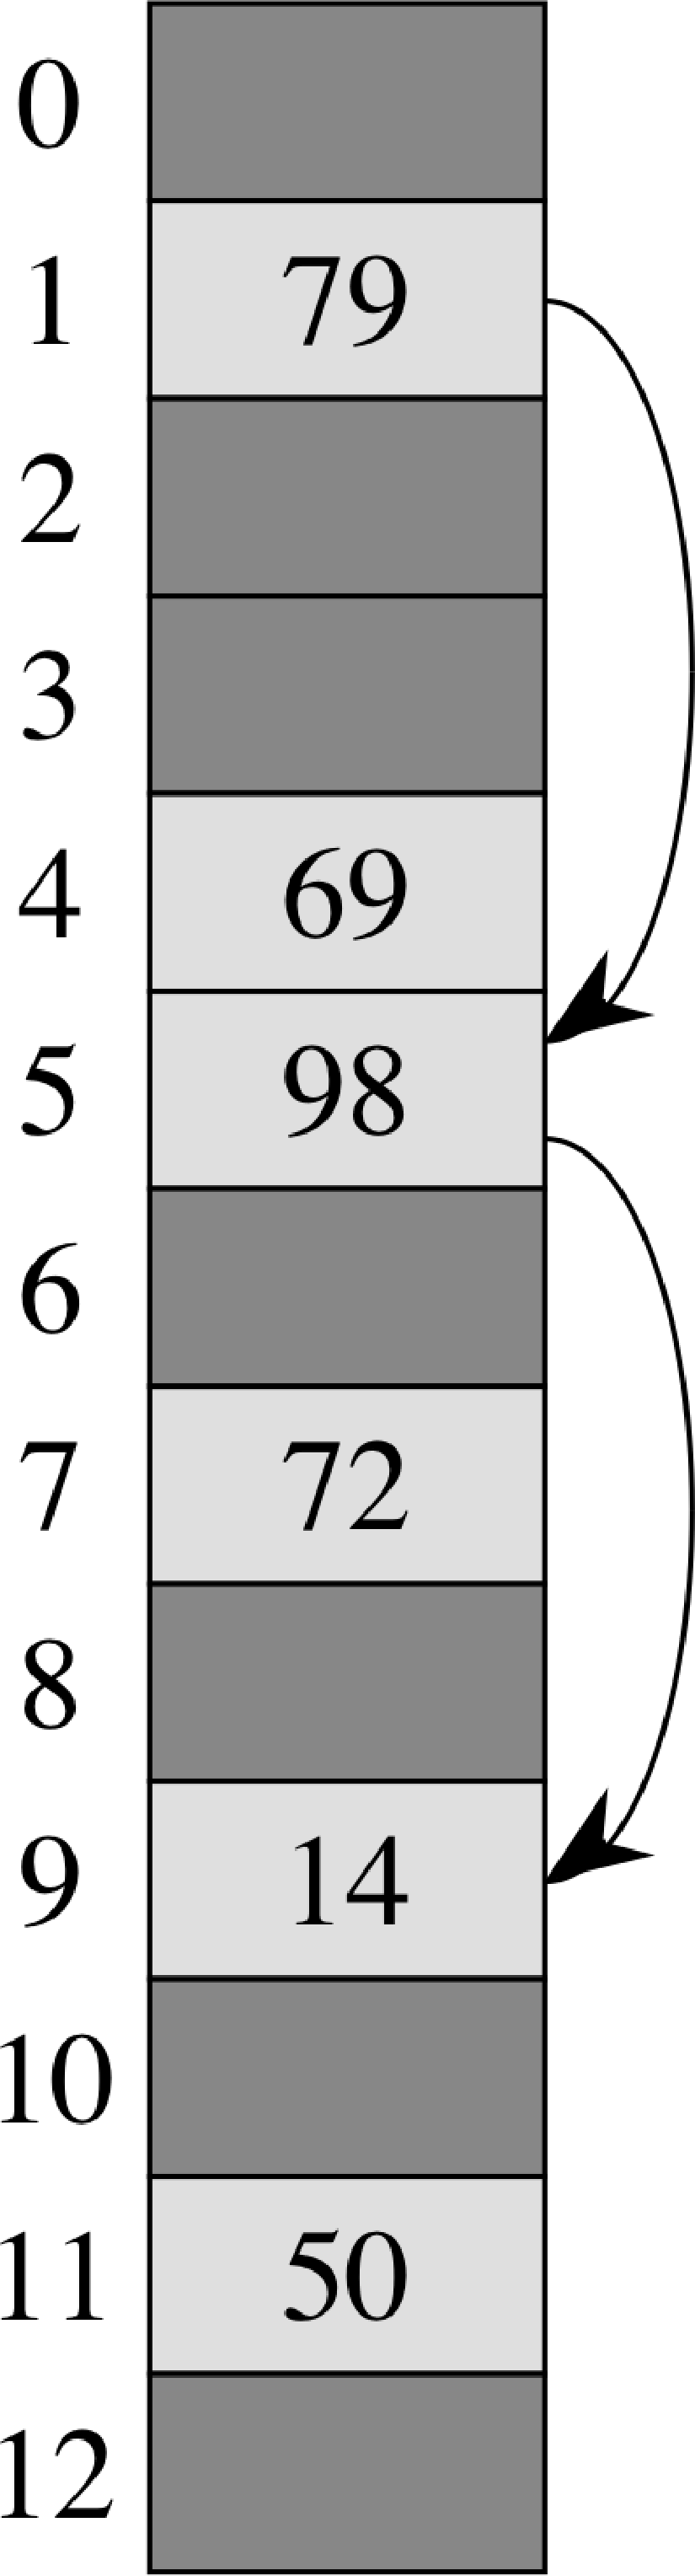
\includegraphics[height=\textheight]{Fig-11-5.pdf}

%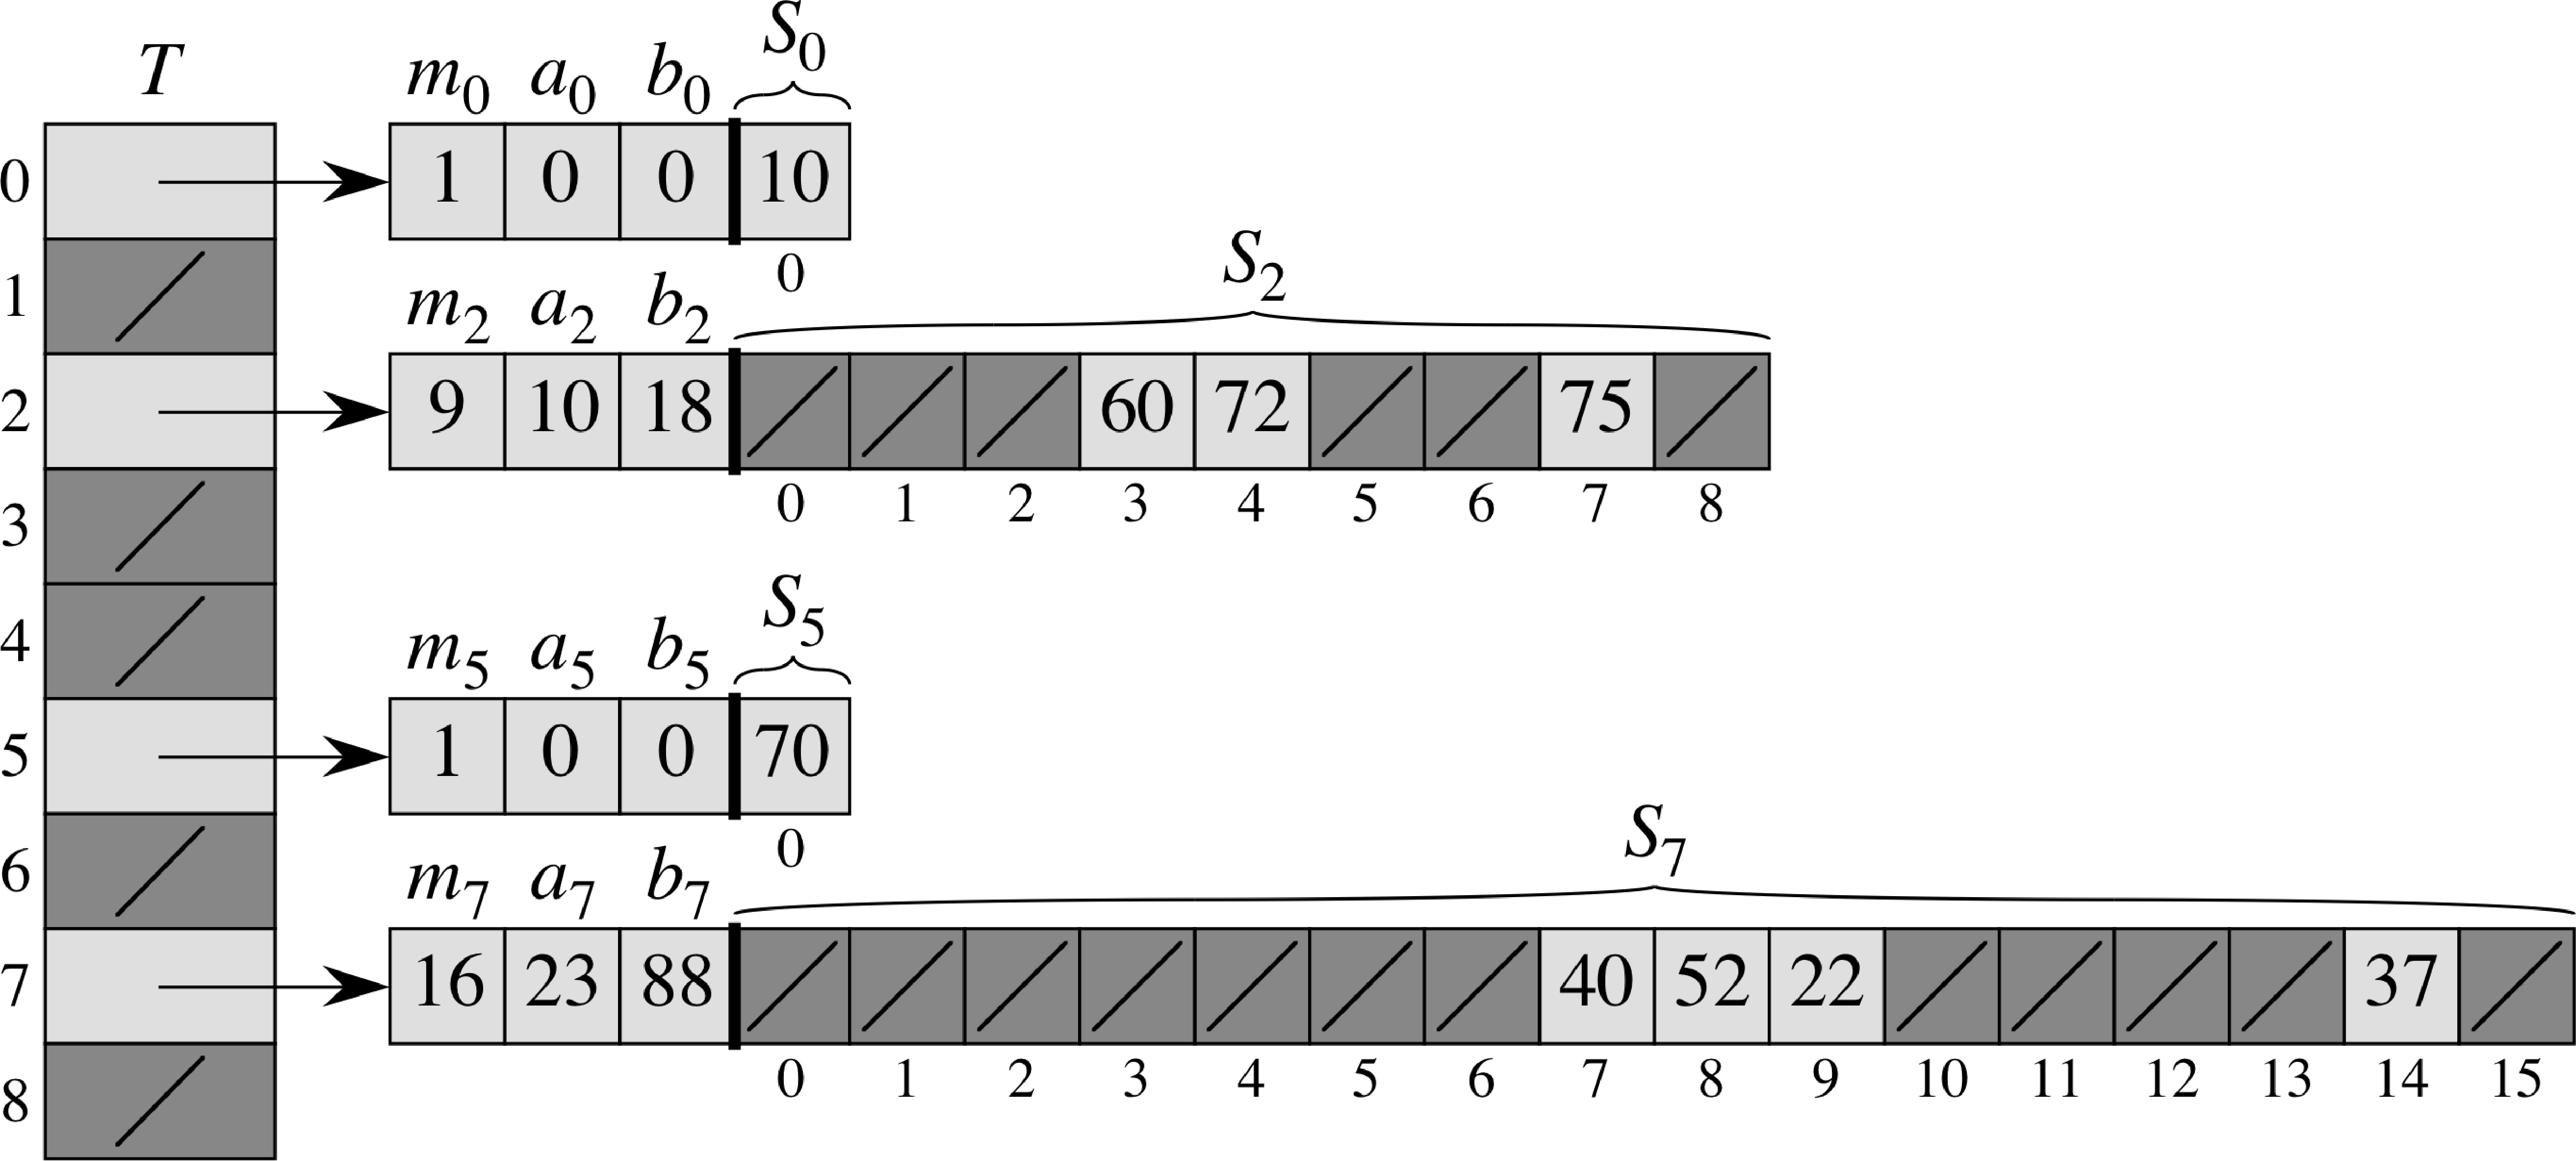
\includegraphics[width=\textwidth]{Fig-11-6.pdf}


\end{document}
